\documentclass{article}
\usepackage{graphicx}
\graphicspath{ {latex/} }
\usepackage{mathtools}
\usepackage{polski}
\usepackage[utf8]{inputenc}

\begin{document}

\title{O krolikach w Polsce}
\author{Michal Krause}

\maketitle

\section{Introduction}

W Polsce nie spotkamy za wiele królików, ale jeżeli już spotkamy to będzie to Królik Europejski. Występujący w zachodniej części kraju szarak mierzy od 35 do 45 cm i waży od półtora do trzech kilogramów, i z Wikipedii: "Grzbiet ma ubarwienie brązowoszare, stalowoszare lub żółtoszare, spód ciała jest białoszary lub popielatoszary. Krótki ogon jest od góry czarny, od spodu biały. Niektórzy mogą pomylić z zającem szarakiem, gdyż przypomina go nieco swoim wyglądem, lecz z powodu trzymania tylnych kończyn blisko siebie, sprawia wrażenie bardziej krępego. Końce uszu królika są brązowe, a szaraka czarne. Zając szarak ma dłuższe uszy i dłuższe tylne nogi. Króliki swoim słodkim zachowaniem i miękkim futerkiem zaskarbiły sobie miłość wielu Polaków i zamieszkują w ich domach w klatkach, tak więc można śmiało stwierdzić, że

\begin{equation}
\Delta x\_\text{Miłość} = \sum x\_\text{SłodkieZachowanie} + x\_\text{MiękkieFuterko}
\end{equation}

\subsection{Systematyka}

Systematyka:
\begin{itemize}
\item O. cuniculus algirus
\item O. cuniculus brachyotus
\item O. cuniculus cnossius
\item O. cuniculus cuniculus
\item O. cuniculus habetensis
\item O. cuniculus huxleyi
\end{itemize}

\subsection{Dzikie a udomowione}
\begin{table}[]
\centering
\begin{tabular}{lllll}
                  & Dzikie                & Udomowione              &  &  \\
Dieta             & Gałązki, zioła, trawy & Pasza, granulki, łodygi &  &  \\
Różnice w budowie & Ok. 20\% wiekszy mózg & Zmniejszone uszy        &  &  \\
                  &                       &                         &  & 
\end{tabular}
\end{table}
\ref{tabela}

\section{Zdjęcia}

Zdjęcia, czyli to na co wszyscy czekali. Przygotowałem dla was dzisiaj trzy zdjęcia uroczych króliczków, oto one:

\begin{enumerate}

\item 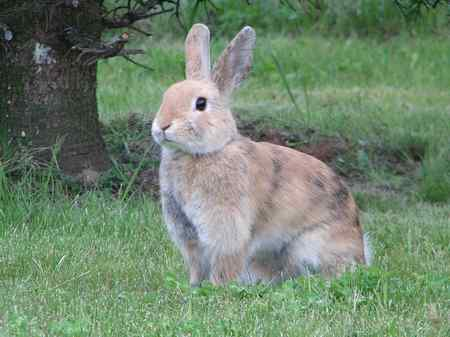
\includegraphics{krolik1}
\item 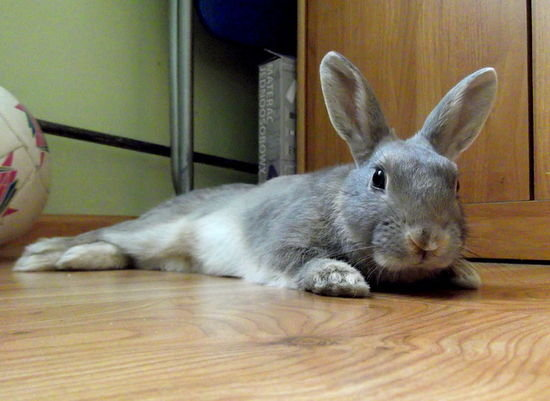
\includegraphics{krolik2}
\item 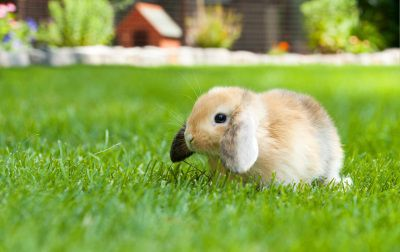
\includegraphics{krolik3}

\end{enumerate}
\ref{zdjecia}


\begin{thebibliography}{9}

\bibitem{Wikipedia}
Wikipedia
\textit{Strona Królik Europejski}
\label{equat}

\bibitem{UszataStrona}
UszataStrona.pl
\textit{FAQ Uszatastrona.pl}
\label{tabela}

\bibitem{Google Graphics}
Grafika Google
\textit{Zdjęcia Królików}
\label{zdjecia}

\end{thebibliography}
\end{document}